\documentclass[a4paper,12pt]{article}
\usepackage[utf8]{inputenc}
\usepackage[spanish]{babel}
\usepackage{amsmath}
\usepackage{amsfonts}
\usepackage{amssymb}
\usepackage{multirow}
%\usepackage{makeidx}
\usepackage{graphicx}
\usepackage{fancyhdr}
\usepackage{hyperref}
\usepackage{float}
\usepackage{color}
\usepackage{booktabs}
\definecolor{azulUC3M}{RGB}{0,0,102}
\definecolor{gray97}{gray}{.97}
\definecolor{gray75}{gray}{.75}
\definecolor{gray45}{gray}{.45}
\usepackage{listings}
\lstset{ frame=Ltb,
     framerule=0pt,
     aboveskip=0.5cm,
     framextopmargin=3pt,
     framexbottommargin=3pt,
     framexleftmargin=0.4cm,
     framesep=0pt,
     rulesep=.4pt,
     backgroundcolor=\color{gray97},
     rulesepcolor=\color{black},
     %
     stringstyle=\ttfamily,
     showstringspaces = false,
     basicstyle=\small\ttfamily,
     commentstyle=\color{gray45},
     keywordstyle=\bfseries,
     %
     numbers=left,
     numbersep=15pt,
     numberstyle=\tiny,
     numberfirstline = false,
     breaklines=true,
   }
 
% minimizar fragmentado de listados
\lstnewenvironment{listing}[1][]
   {\lstset{#1}\pagebreak[0]}{\pagebreak[0]}
 
\lstdefinestyle{consola}
   {basicstyle=\scriptsize\bf\ttfamily,
    backgroundcolor=\color{gray75},
   }
 
\lstdefinestyle{C}
   {language=C,
   }
\usepackage[top=2cm]{geometry}
\pretolerance=2000
\tolerance=3000
\setlength{\parindent}{0pt}
\begin{document}

\begin{titlepage}
\begin{sffamily}
\color{azulUC3M}
\begin{center}
%\vspace*{-1cm}
\begin{figure}[htb]
\begin{center}
\vspace*{0.6cm}

\includegraphics[width=15cm]{imagenes/Portada_Logo.png}
\vspace*{1.6cm}
\end{center}
\end{figure}
\begin{LARGE}
Grado en Ingeniería Informática \\%completar el nombre del grado
2020/2021 \\%indicar el curso académico
\vspace*{2cm}
\textsl{Prácticas en empresa}\\
\end{LARGE}

\begin{huge}
\textbf{Grupo Go Optimizations \\  Capital Certainty \\ Global Incubator} \\
\rule{80mm}{0.1mm}\\
\vspace*{1cm}
Javier Alonso Mencía % cada autor con \\ 
\end{huge}

\vspace*{1cm}
\begin{Large}
Tutores\\
UC3M: Álvaro Pariente Alonso  \\
Empresa: José Sanz Polo

\end{Large}
\end{center}
\vspace*{1cm}
\color{black}
\begin{figure}
\begin{center}

\includegraphics[scale=0.7]{logo.png}\\
\end{center}
\end{figure}


\end{sffamily}
\end{titlepage}


\pagestyle{fancy}
\fancyhead{} % Clear all header fields
\setlength\headheight{21.2pt}
\lhead{\hspace*{-0.3cm}\raisebox{-0.3\height}{
\includegraphics[scale=1]{imagenes/Interior_Logo.png}}}
\rhead{\color{azulUC3M} Prácticas en empresa} %Poner encabezado

\renewcommand{\tablename}{\textbf{Tabla}} %para poner la palabra en mayusucula
\renewcommand{\figurename}{\textbf{Figure}} % para poner la palabra en mayuscula
\renewcommand{\listtablename}{Índice de tablas}

\newpage

\tableofcontents

\newpage


%Para imagenes
%\begin{figure}[H]
%\centering
%\includegraphics[scale=0.8]{imagenes/*.png}
%\caption{}
%\end{figure}

\newpage



\section{Información relevante}

\paragraph{Datos personales}\mbox{}\\
\begin{table}[H]
\begin{tabular}{@{}lll@{}}
Nombre   & \mbox{} & Javier Alonso Mencía      \\
NIA    & \mbox{} & 100383503                 \\
Grado & \mbox{\phantom{adrfgsegkrdthrs}} & Ingeniería Informática     \\
Email  & \mbox{} & 100383503@alumnos.uc3m.es
\end{tabular}
\end{table}

\paragraph{Información de la empresa}\mbox{}\\
\begin{table}[H]
\begin{tabular}{@{}lll@{}}
Nombre  &                                       & Grupo Go Optimizations (Global Incubator) \\
Tutor &                                    & José Sanz Polo                                   \\
Email & \mbox{\phantom{adrfgsewefaefrtz}} &  jose.sanz@capitalcertainty.com                      \\
Teléfono & \mbox{\phantom{adrfgsewefaefrtz}} &  
625612788
\end{tabular}
\end{table}

\paragraph{Información sobre las prácticas}\mbox{}\\
\begin{table}[H]
\begin{tabular}{@{}lll@{}}
Periodo &  \mbox{\phantom{dwdwdwdw}}                                  & 08/06/2020 - 31/08/2020 \\
Horas diarias &   \mbox{\phantom{dwdwdwdw}}                               & 8h (Lunes - Viernes)
\\
Horas totales &  \mbox{\phantom{dwdwdwdw}}                                 & \textbf{488h (6 ECTS)}    
\\
\end{tabular}
\end{table}

\newpage

\section{Introducción}

Me gustaría empezar este documento mencionando unas prácticas que se iban a realizar este verano en una empresa situada en China de Impresión 3D llamada ANYCUBIC, pero debido a la grave situación en la que todavía nos encontramos, se decidió cancelarlas y buscar una alternativa cercana a mi domicilio. \\
\\
Considero que hubiese sido una experiencia muy enriquecedora en cuanto a conocimientos y cultura, pero en estos momentos la salud es más importante.\\
\\
En este documento se recoge información relevante relacionada con las prácticas que he podido realizar durante este verano en la empresa Global Incubator, la cual forma parte de GRUPO GO OPTIMIZATIONS, S.L. Dicho grupo engloba varias pequeñas empresas de varios ámbitos tecnológicos. Cabe mencionar que este grupo ha migrado este año su nombre a Capital Certainty, aunque en el convenio que tiene con la UC3M sigue apareciendo el nombre anterior.\\
\\
La información que se expone está relacionada con los conocimientos obtenidos, cómo se han puesto en práctica dichos conocimientos en un proyecto real, mis aportes en la empresa, la relación de estas prácticas con mis estudios universitarios y las conclusiones sobre mi primera experiencia en el mercado laboral.\\
\\
Finalizo esta introducción recalcando que se ha teletrabajado durante todo el periodo de prácticas, pero esto no ha impedido mantener un ambiente laboral debido a las numerosas reuniones y sistema de control de tareas que se ha llevado.\\




\section{Prácticas}
Dentro de Global Incubator se realizan varios proyectos simultaneamente.
Estas prácticas han sido realizadas dentro de un equipo dedicado específicamente a un proyecto web para el banco Santander. 
Este equipo a su vez está dividido en varios subequipos, pues este proyecto web engloba varios campos a tratas, desde diseño UX, hasta Front, Back, Security, etc.
En mi caso en particular, participo en el subequipo de Front del equipo dedicado al proyecto para el banco Santander.\\
\\ 
En este proyecto para el banco Santander he obtenido nuevos conocimientos y puesto en uso algunas tecnologías aprendidas en la universidad.
A continuación se indican los objetivos principales extraidos de estas prácticas.

\subsection{Objetivos}

Los principales objetivos de estas prácticas fueron los siguientes:
\begin{itemize}
\item \textbf{Conocer y participar en un ambiente laboral}: Estas prácticas corresponden con mi primera experiencia laboral, por lo que lo considero un objetivo muy importante. No se puede comparar la vida universitaria con el mundo laboral pues existe una brecha notable.\\

En primer lugar, cabe destacar la participación en reuniones diarias donde se compartía con el resto del equipo las tareas realizadas. La empresa seguía la metodología SCRUM, pues consideran que es muy útil para no dejar a nadie atras si existe algún bloqueo de desarrollo, además de ver en que fase del proyecto se encuentra cada subgrupo.

\item \textbf{Aprendizaje y puesta en práctica de tecnologías Frontend}:
En la universidad he aprendido varias tecnologías aplicadas al desarrollo web como son HTML, CSS, Javascript, TypeScript y
Angular. \\
\\Sin embargo, en este proyecto web para el banco Santander se usa React, por lo que ha sido necesario aprender esta nueva tecnología que se asemeja a Angular pero tiene diferencias notables. Además, la profundidad con la que he podido aprender React ha sido mucho mayor que la que obtuve con Angular en mi carrera, pues aquí se ha podido aplicar a un proyecto mucho mayor.\\
React funciona usando componentes que se podrían explicar como partes de una página. Por ejemplo, el header de una web podría ser por si solo un componente, una columna que muestre el tiempo meteorológico podría ser otro componente, etc. Esto permite tener una mayor flexibilidad a la hora de editar, cambiar o mover componentes. Cada componente incluye el código HTML, estilos en CSS y la lógica usando JavaScript (por ejemplo, qué ocurre al pulsar un botón).

\item \textbf{Aprendizaje y puesta en práctica de tecnologías Backend}:
Respecto a tecnologías Backend no tenía conocimientos previos antes de comenzar las prácticas. Para no extenderme demasiado en la explicación, el Backend consiste en aquellos servicios que se encargan de acceder a un servidor donde se almacena información específica y llevarla hasta el Frontend donde se usará para mostrar algunos datos.\\
Por otra parte, también se usa para comunicar la interacción del usuario con el Frontend con el servidor para intercambiar información.\\
\\
Todo el Backend está basado en NodeJS. Además de usar dicha tecnología, se usó una herramienta muy útil para este tipo de tareas llamada Postman que permite comprobar el funcionamiendo del Backend rápidamente para encontrar problemas en los servicios REST.

\begin{figure}[H]
\centering

\includegraphics[scale=0.7]{react-node.png}
\caption{Tecnologías web usadas en el proyecto}
\end{figure}

La imagen que se muestra a continuación puede ayudar a comprender las dimensiones del proyecto. En mi caso, me encontraría dentro de la parte de Frontend y Backend usando tecnologías React situado en la zona izquierda superior de la imagen.

\begin{figure}[H]
\centering
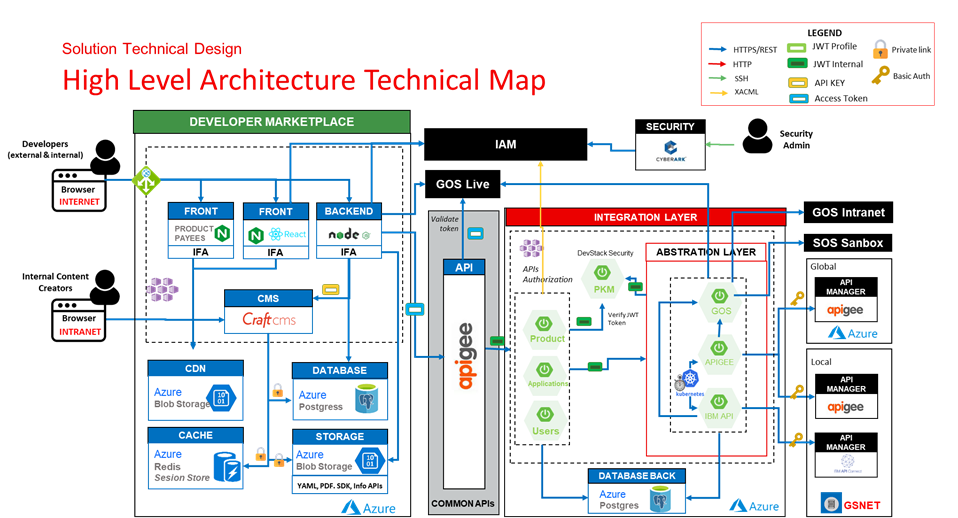
\includegraphics[scale=0.4]{mapa.png}
\caption{Mapa del proyecto web para el banco Santander}
\end{figure}

\end{itemize}

\subsection{Trabajo realizado}

En esta sección se explica con detalle el proyecto web para el Banco Santander en el que he tenido la oportunidad de participar.

\subsubsection{Descripción del proyecto}

Este proyecto consiste en crear una plataforma web para desarrolladores donde el Banco Santander les ofrece una serie de herramientas para crear APIs que posteriormente puedan ser usadas por otros usuarios a través de subscripciones de pago. En la plataforma, existen organizaciones a las que se pueden unir usuarios y a su vez en cada organización el usuario puede crear aplicaciones.\\
\\
Además, aunque el Banco Santander es un banco español, tiene sedes en diversos países. Por esa razón, este proyecto va destinado a varios países entre los que destacan Brasil, Reino Unido, Estados Unidos y España.\\
\\
En un principio, el proyecto se está desarrollando en inglés, aunque el primer país donde entrará en funcionamiento será en Brasil. Por esa razón, por ahora se han incorporado los idiomas inglés y portugués por ahora. \\
Además, las vistas del proyecto en las que he participado van destinadas a Brasil.\\
\\
Es un proyecto relativamente grande pues dentro de Global Incubator participan varios equipos de Frontend, Backend y Security. Cabe mencionar que en este proyecto participan otras empresas como Bloomreach. Esta empresa se dedica a crear CMS, es decir, gestor de contenidos para webs. Si el lector desconoce lo que es un CMS, se podría utilizar como referencia el panel de Wordpress para entender lo que es un CMS. Sin embargo, esta parte no nos incumbe debido a que ha sido externalizada por el banco Santander a otra empresa.\\
\\
También es importante mencionar cómo se controlan los avances en el proyecto. Varias personas del banco Santander realizan reuniones diarias o semanales con los equipos de Global Incubator en las que he podido participar. En dicha reuniones mi equipo muestra problemas, retrasos y tareas que han sido completadas. Por otro lado, el project manager del Santander se encarga de controlar como va el desarrollo intentando meter un poco de presión para que las tareas que tienen problemas vayan saliendo lo antes posible.\\
\\
Hay que entender que un project manager no siempre tiene conocimientos de desarrollo de software, por lo que he podido observar un cierto desconocimiento a la hora de calcular las estimaciones de tiempo que el project manager cree que puede necesitar una tarea para ser completada.\\

Para terminar esta introducción, me gustaría destacar que existían dos maneras para controlar el desarrollo del proyecto. El proyecto está subdividido en tareas y a cada persona se le asignan unas tareas en cada planificación que se lleva a cabo cada dos semanas.\\
El proyecto se controlaba de manera interna dentro de la propia Global Incubator a través de una página web propia donde cada persona anotaba sus tareas y el tiempo que le dedicaba a cada tarea.\\
\\
Por otra parte, para controlar el proyecto de manera externa junto al equipo del banco Santander se utilizaba una herramienta llamada Jira donde los representantes de cada equipo de Global Incubator se encargaban de indicar si una tarea estaba bloqueada, en proceso, lista para testearla o completada.\\
En mi caso no fue posible acceder a dicha herramienta aunque en las reuniones diarias pude observar su funcionamiento y comprobar lo útil que era.


\subsubsection{Contribución en el proyecto}

Mi contribución en el proyecto reside principalmente en dos partes que se describen a continuación.

\begin{itemize}
    \item \textbf{Realización de vistas en Frontend}: Se ha desarrollado el HTML, CSS y JavaScript usando React en las vistas siguientes.
    \begin{itemize}
        \item \textbf{Página FAQS (preguntas frecuentes)}: La vista de preguntas frecuentes en un principio no se le suele dar mucha importancia. Sin embargo, es una de las páginas más importantes de cualquier web a la que los usuarios acceden cuando están realizando una toma de contacto en una página y tienen dudas o problemas sobre como realizar alguna tarea o función.\\
        \\
        Me gustaría ilustrar con la vista realizada para que el lector tenga en todo momento presente la vista según se van explicando las partes de las que se compone. En cualquier vista, el desarrollo inicial se realiza con información irrelevante. Una vez acabado, se incluye la información final que el cliente requiere a través de servicios Backend.
        \begin{figure}[H]
            \centering
            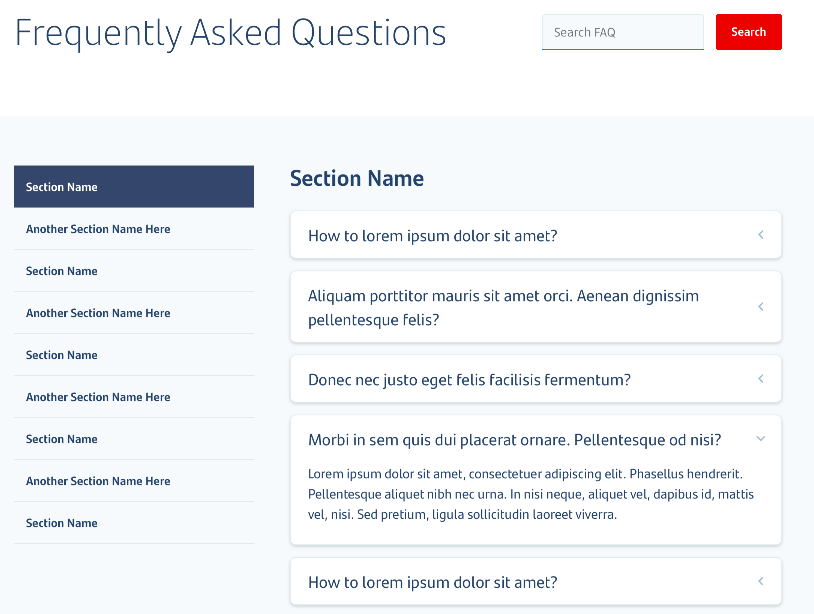
\includegraphics[scale=0.9]{faq.PNG}
            \caption{Página FAQS}
            \label{fig:my_label}
        \end{figure}
        
        El proceso para llevar a cabo esta vista fue dividirla en componentes que interaccionan entre ellos. Puede parece una vista simple pero llevó casi tres semanas de trabajo convirtiéndola en una de las páginas más complejas que he realizado durante mis prácticas. Esto fue debido a los continuos cambios de diseño y requisitos y se iban incluyendo según iba realizando la vista.\\
        \\Se distinguen tres partes principales en esta vista, como son la parte de búsqueda, el menú lateral izquierdo para moverse entre secciones y el cuerpo con las preguntas y respuestas para cada seccioón.\\
        Respecto a la parte de la búsqueda, corresponde al encabezado de la vista incluyendo el título de la misma. \\
        Esta parte tuvo su dificultad pues en los requisitos de la búsqueda se pedía que se filtrasen todas las preguntas de todas las secciones. Posteriormente se debían renderizar únicamente las preguntas encontradas sin incluir las secciones a su izquierda.\\
        \\Respecto a la parte del menú de secciones, fue una parte relativamente sencilla porque solo se necesitaba conocer a que sección quería desplazarse el usuario.
        Finalmente, el componente de preguntas de la sección tuvo su complejidad pues cada respuesta a una pregunta aparecía como un desplegable. Gracias a varias librerías se pudo resolver facilmente.\\
        \\
        Además, otro requisito para esta parte era contar con un único desplegable abierto cada vez. Es decir, si había un desplegable abierto y el usuario quería abrir otro nuevo, el anterior debía cerrarse.\\
        Esta parte fue bastante díficil pues el requisito fue añadido una vez que se acabó la versión inicial de la vista.\\
        
        Una vez que se completó toda la parte del HTML y la parte lógica con JavaScript, era necesario incluir estilos. Esta parte fue compleja pues la página debe ser responsive, es decir, debe estar adaptada para pantallas de móviles, tablets y ordenadores. Fue una parte que llevó también bastante tiempo por nuevos cambios que se introdujeron en el diseño pero finalmente se pudo completar con apoyo de otros compañeros de diseño del equipo.\\
        \\
        La última parte de esta vista consistió en incluir la información real del cliente en la vista que se realizó gracias al servicio Backend creado que se explica en la sección correspondiente.
        
        \item \textbf{Página Información Legal}: Está página incluye a su vez las vistas de Términos y Condiciones y la Política de Cookies.\\
        Estas páginas son necesarias en cualquier página web de hoy en día debido a las legislaciones de cada país.\\
        \\
        A continuación se muestra una parte de la vista.
        \begin{figure}[H]
            \centering
            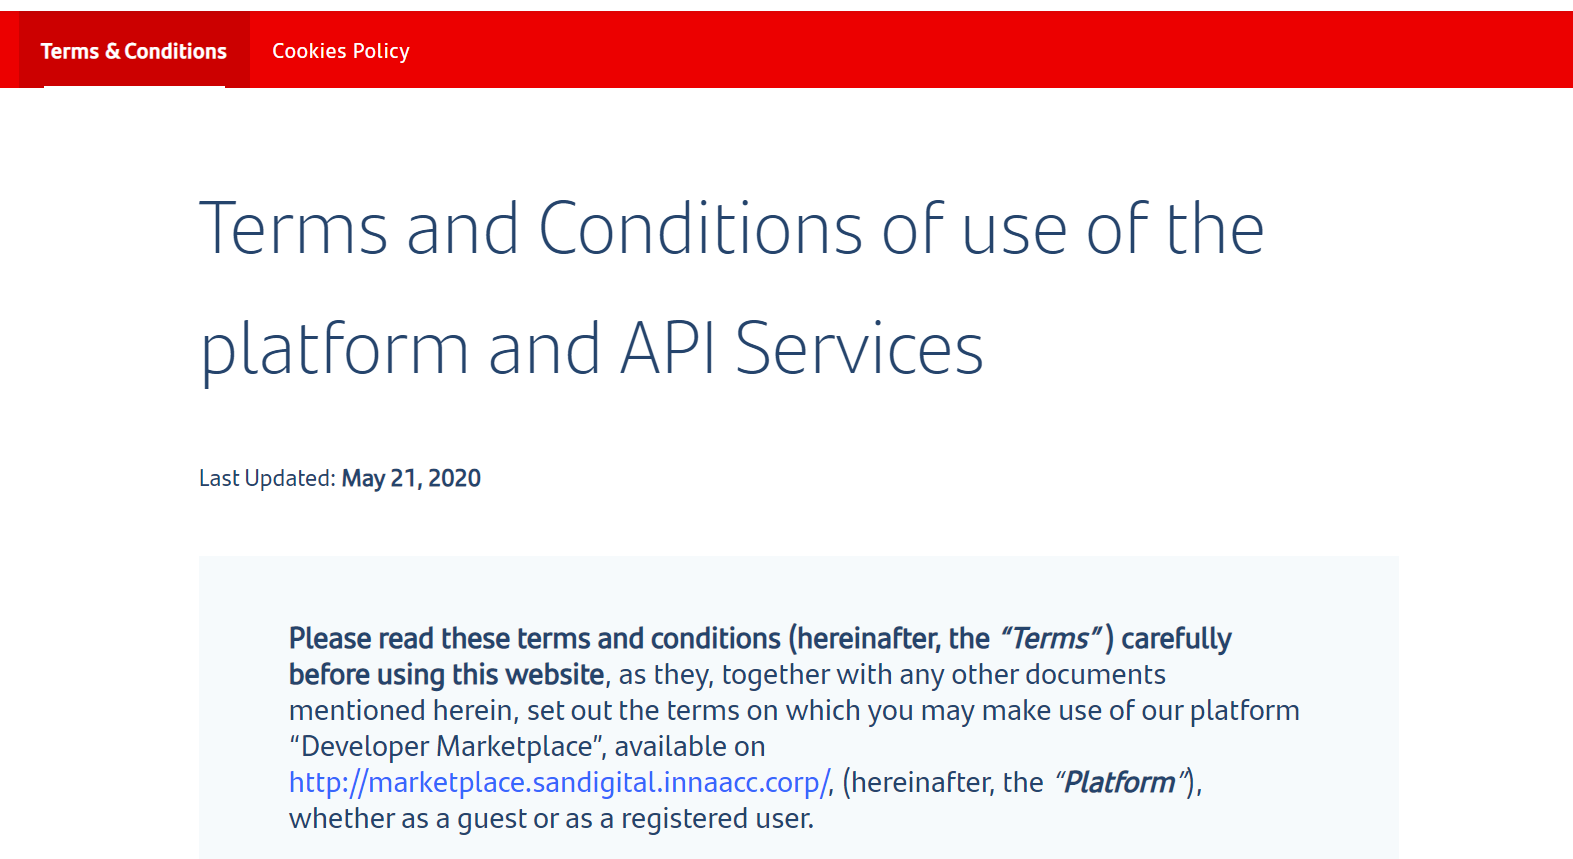
\includegraphics[scale=0.5]{legal.PNG}
            \caption{Página Información Legal}
            \label{fig:my_label}
        \end{figure}
        
        Esta vista consta de tres partes bien definidos. La parte superior que permite intercambiar entre las vistas de Términos y Condiciones y la de Política de Cookies.\\
        \\
        Una vez que esa parte estaba completada, únicamente era necesario crear dos componentes más para incluir las dos vistas principales de la página. Tanto Términos y Condiciones como la Política de Cookies son páginas muy similares en diseño. Por esa razón se decidió completar primero una de ellas para después poder replicarla y cambiar únicamente su contendido.\\
        \\
        La parte compleja de esta vista reside en conseguir los mismos estilos que requiere el cliente. Una vez cumplido ese requisito, la vista no tuvo muchos problemas salvo algunos estilos especiales para adaptarse a diversas resoluciones de pantalla.
        
        \item \textbf{Footer de la página}: Esta parte de la página corresponde al pie de página. Es visible desde todas las páginas de la plataforma.\\
        \\
        Como se puede observar a continuación, esta formada por tres partes principales con diferentes colores de fondo.
        \begin{figure}[H]
            \centering
            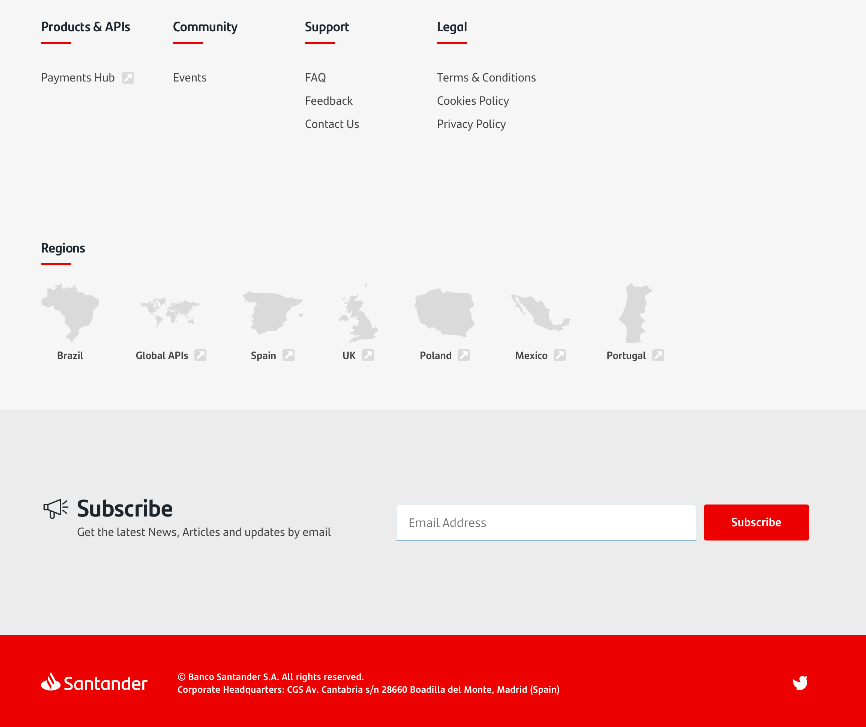
\includegraphics[scale=0.7]{footer.PNG}
            \caption{Footer}
            \label{fig:my_label}
        \end{figure}
        
        Esta parte de la página tiene mucha importancia, pues como se ha mencionado antes, es visible desde cualquier parte de la página. Está formada por tres partes. La primera parte incluye diversas secciones que permiten acceder a páginas específicas como las FAQS, Términos y Condiciones, Contactar con soporte, etc.\\
        También se puede observar una sección de Regiones. Si el lector lo recuerda, se comentó que está plataforma iba a ser usada en diferentes países donde el banco Santander tiene sede. Por esa razón aparece esta sección.\\
        \\
        A continuación aparece una zona donde el usuario puede subscribirse con su correo electrónico a una Newsletter para recibir información relevante.\\
        \\
        En la parte inferior encontramos información sobre la localización de la sede del Banco Santander así como un acceso a sus redes sociales.\\
        \\
        Esta vista no cuenta con mucha Lógica, sino que destaca más por sus estilos en CSS. La vista fue subdividida en las tres secciones que se han comentando y posteriormente se unieron para formar un único bloque.\\
        Una vez creado el HTML, se continuó añadiendo estilos. Esta parte tuvo mucha complicación debido a las grandes diferencias que había entre la versión para ordenador y la versión móvil que incluye menus desplegables. Es esta parte se contó ayuda externa del equipo para poder resolver ciertos problemas que requerían un nivel más elevado de conociminetos.\\
        
        \item \textbf{Página para eliminar o editar organizaciones}: Esta vista permite a los usuarios creadores de una Organización poder eliminarla siempre y cuando no tengan activa ninguna subscripción activa en alguna aplicación de la organización.\\
        \\
        Esta página tiene grandes complicaciones debido a que cuenta con varios pasos para poder realizar el proceso. Se explica brevemente a continuación acompañándolo de sus capturas correspondientes para permitir al usuario crear una imgen mental del proceso.\\
        \\
        En primer lugar, el creador de una organización desea eliminarla accediendo a una página donde debe eliminar todas las suscripciones activas que tenga para cualquier aplicación de dicha organización.
        \begin{figure}[H]
            \centering
            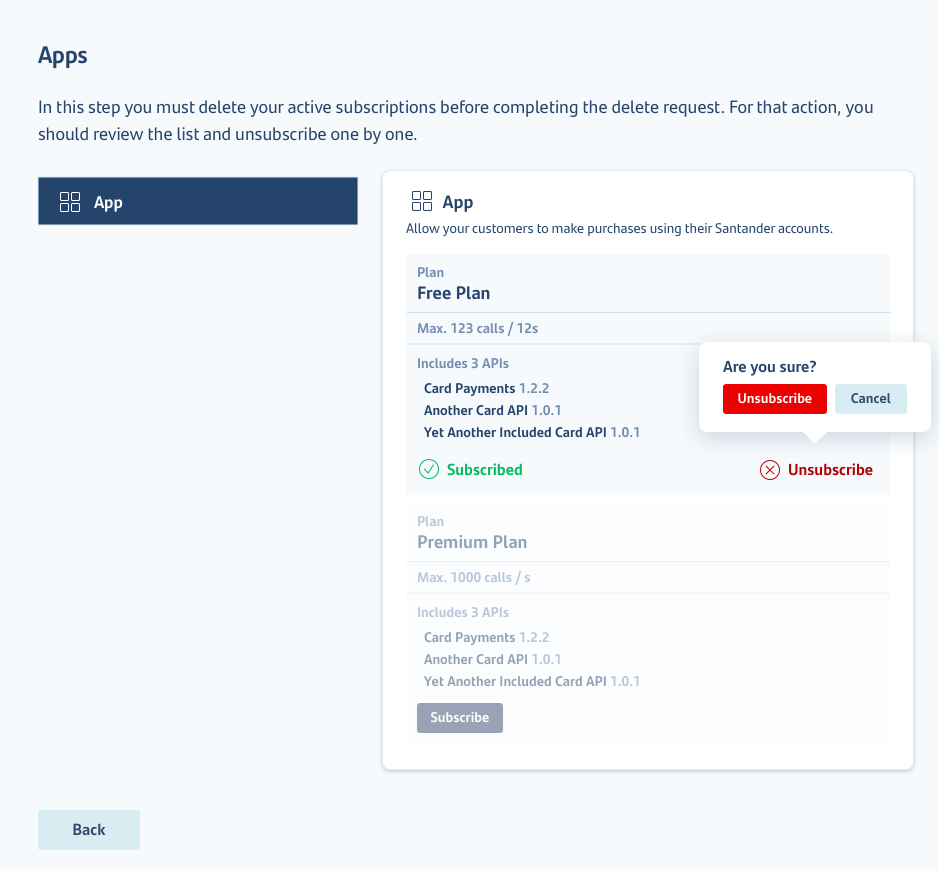
\includegraphics[scale=0.7]{appsSub.PNG}
            \caption{Página para Eliminar Subscripciones Aplicaciones}
            \label{fig:my_label}
        \end{figure}
        
        Esta página no fue creada desde cero, pues exisitía una página similar que se podía reusar. Sin embargo, toda la parte de la lógica para seleccionar diferentes aplicaciones y recopilar del servicio correspondiente toda la información de cada aplicación si que fue llevada a cabo.\\
        \\
        Es importante mencionar que en la acción de eliminar un plan se incluye un servicio que se conecta con el servidor para poder aplicar los cambios que desea el usuario.\\
        El lector puede pensar que sería más sencillo dar la opción al usuario de eliminar todas las subscripciones con tan solo pulsar un botón. Sin embargo, estas suscripciones puede ser de pago y tener un coste muy elevado. Por esa razón se realizó este diseño.\\
        Durante cada interacción en la que el usuario elimina las subscripciones activas de cada aplicación, estas van desapareciendo hasta que no queda ninguna y aparece la siguiente vista.\\
        \\
        Esta vista es el paso final para eliminar una organización. Aparece cuando ya no quedan aplicaciones con subscripciones activas.
        
        \begin{figure}[H]
            \centering
            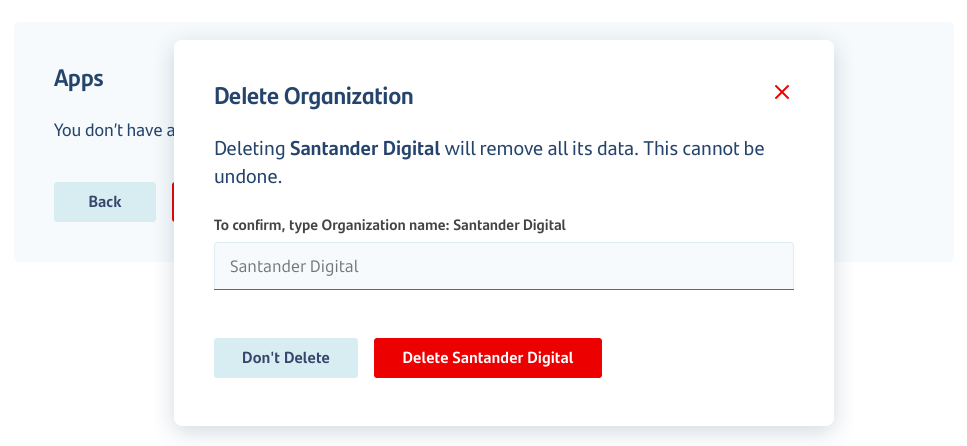
\includegraphics[scale=0.7]{deleteorg.PNG}
            \caption{Modal Eliminar Organización}
            \label{fig:my_label}
        \end{figure}
        
        Consiste en un modal sencillo donde el usuario debe escribir el nombre de la organización para finalmente ser elminada. Desde un punto de análisis de diseño UX, es una manera de ser consciente de que el usuario realmente quiere eliminar dicha organización y no está cometiendo un error con la organización.
        
        La principal dificultad de esta vista reside en la lógica para comunicar los diversos componentes entre ellos. Una vez conseguido esta parte, el resto de detalles y retoques de estilos para adaptarse a diferentes resoluciones fue bastante sencillo.
        
    \end{itemize}
    
    \item \textbf{Realización de servicios en Backend del Frontend}: Se han desarrollado una serie de servicios que permiten pedir información a un servidor de Microsoft Azure de manera segura por diversas capas de seguridad y que es usada en la vistas del Frontend. Esta parte es díficil de representar de manera escrita pues es código que se usa como intermediario para conectar el Frontend con el servidor.
    \begin{itemize}
        \item \textbf{Servicio para editar el nombre de una organización}: Este servicio permite a un usuario de la plataforma modificar el nombre de una organización. Dicho servicio recibe el nuevo nombre que el usuario y lo comunica al servidor para que realice el nombre. \\
        Si se realiza de manera efectiva, el usuario lo podrá ver actualizado en su plataforma. Si existe algún error inesperado en el servicio, el usuario también podrá ver qué problema ha ocurrido.
        
        \item \textbf{Servicio para recibir información para la página de FAQS}: Este servicio consiste en recopilar información desde el CMS con las secciones y preguntas frecuentes que se desean mostrar en la página web.\\
        La dificultad de esta tarea residió en el formato con el que se recibe toda la información, pues debe tener un formato similar al usado en el Frontend de las FAQS para poder mostrar el contenido sin errores. Después de arreglar algunos problemas iniciales de formato, todo funcionó correctamente.
        
    \end{itemize}
\end{itemize}

\subsection{Habilidades obtenidas}

Una vez finalizado mi periodo de prácticas, puedo asegurar que he conseguido desarrollar mis habililidades personales y profesionales gracias a esta oportunidad. Algunos puntos destacables que me gustaría destacar son los siguientes:

\begin{itemize}
\item Desarrollo de las capacidades intelectuales: la capacidad de aprender cosas nuevas en poco tiempo y contribuir con ellas a un proyecto global para una empresa grande de una manera activa fue muy interesante. Aprender un nuevo framework para el desarrollo web, contribuir con mis conocimientos adquiridos durante mis años universitarios a un proyecto grande y descubrir que algunas de las tecnologías aprendidas a lo largo de estos años han sido utiles en todos los aspectos fue muy satisfactorio.

\item Mejora de habilidades personales: trabajo en equipo, visión global, comunicación, capacidad de cooperar y ayudar en tareas. Participar en reuniones diarias y mejorar mis habilidades comunicativas se han potenciado a lo largo de estas prácticas. 

\item Primeros pasos en el desarrollo web profesional: hasta este punto mi experiencia en el sector de tecnologías web se limitaba a lo aprendido durante la carrera y lo aprendido por mi cuenta. Es decir, como estudiante no tenía ningún contacto previo con las tecnologías que realmente se usaban en las empresas. Esta experiencia me ha ayudado a ver cómo funciona la industria del desarrollo web a parte de lo que se me ha trasmitido desde la universidad (que resultó ser precisa en bastantes aspectos). Anteriormente había trabajado en otros sectores (impresión 3D), pero mi experiencia dentro del desarrollo web profesional era nula. Sin embargo, esta oportunidad me ha permitido crecer profesionalmente.
\end{itemize}

\newpage


\subsection{Sugerencias}

Gracias a esta experiencia, me gustaría aportar una serie de recomendaciones para incluir en mi grado de Informática que podría ser de gran utilidad para ayudar a futuros estudiantes en el mundo laboral: 
\begin{itemize}
\item \textbf{Ofrecer un mayor soporte para el desarrollo web durante el grado}: Hasta el tercer año del grado de informática no se comienza a introducir el desarrollo web. Entiendo que es un tema delicado pues no es solo programar, sino que necesita un estudio de las interfaces, usuarios, etc. \\
\\
Sin embargo, creo que hoy en día es necesario que el estudiante de informática conozca JavaScript debido a su gran utilidad, no solamente para el desarrollo web. Mi propuesta sería añadir una asignatura en segundo donde se viesen con mas profundidad los lenguajes básicos, empezando por HTML, CSS y JavaScript, pero con mucha profundidad. \\
\\Actualmente existe una asignatura donde se explican dichos lenguages pero con poca profundidaz y el estudiante siente que su conocimiento no ha aumentado mucho.
\item \textbf{Actualizarse a entornos web usados en empresas}: En la carrera se me presentó Angular como framework para el desarrollo web. Es un buen framework aunque por mi experiencia en una empresa, se usa más a menudo React. Es cierto que ambas tecnologías tienes su puntos positivos y negativos, pero considero que es más útil para el estudiante aprender tecnologías que usará una vez acabada la carrera.\\
\\
No me gustaría quitarte prestigio a Angular, pero mi razonamiento puede tener origen en una falta de profundidaz a la hora de aprender dicha tecnología. En mis prácticas fui capaz de aprender React de manera avanzada en 2 semanas con un curso intensivo. \\
\\
En 1 mes creo que no sería complicado que el estudiante aprendiese mejor Angular. Una de mis propuestas sería revisar la manera en la que se está impartiendo o incluso cambiar a otras tecnologías como React y apoyarse de cursos online antes que dejar al estudiante buscar documentación por su cuenta y cometer errores en el proceso.
\item \textbf{Control de versiones con GIT}: Git es la mejor tecnología usada a día de hoy para controlar versiones de software. Sin embargo, en la carrera no se explica al estudiante nada sobre ella y debe ser el propio estudiante el que por sus propios medios ponga el interés en aprender dicha herramienta.. \\
\\
En el primer o segundo curso de programación considero que debería incluirse como temario esta herramienta. En mi caso en particular, no fue hasta este año donde empecé a usarlo recomendado por un compañero de clase. \\
\\
He podido observar en mis prácticas un compañero que se incorporó después que yo a la empresa que justo acabó el grado de Informática en la UC3M. Este compañero desconocía GIT y afirmaba también que se debería ofrecer la posibilidad de aprender GIT en alguna asignatura del grado.\\
\\Dicha herramienta es bastante sencillo y dudo que tomase mucho tiempo aprenderla. Probablemente en un par de semanas el estudiante ya sería capaz de comprender y usar los principales recursos que ofrece de manera autónoma comprendiendo que hace en cada momento. Gracias a este aprendizaje, el estudiante podrá aplicar dichos conocimientos posteriormente a sus propios proyectos de otras asignaturas para mantener un control de versiones y evitar perder código. \\
Por todo este razonamiento, vería necesario incluirla como temario en alguna asignatura.
\end{itemize}


\section{Conclusiones}

Me gustaría finalizar el documento con una breve conclusión sobre la gran utilidad de estas prácticas.\\
\\
Desde que empecé mi carrera en la UC3M, siempre estuve pensando que pasaría al salir de la universidad, pues aunque durante el grado se cursan muchas asignaturas y se obtienen importantes conocimientos, no sabemos si realmente estos conocimientos son útiles en el mundo laboral. \\
\\
Muchos comentan que la universidad aporta únicamente un título que nos permite acceder a puestos de trabajo mejores, y aunque estoy parcialmente de acuerdo, considero que dicha afirmación no es totalmente cierta.\\
\\
Esto es debido a estas prácticas que he podido realizar, donde he podido observar y poner a prueba algunos conocimientos obtenidos durante mis estudios universitarios. Es cierto que existen conocimientos o tecnologías que se aprenden en la universidad y no tienen mucha utilidad en el mercado laboral, ya sea porque son programas desfasados o porque no tienen un fin económico. \\
\\
Sin embargo, gracias a esos conocimientos he podido apreciar que aunque no se usen de manera directa, sirven para crear una base de conocimiento sobre la que posteriormente se añadirán otros nuevos. \\
\\
En el caso de la Informática, es un mundo muy extenso que se encuentra en constante avance. Esto provoca que sea necesario aprender nuevas tecnologías a menudo para poder afrontar nuevos problemas.\\
\\
Yo mismo he podido experimentar de primera mano dichas afirmaciones, pues aunque en la universidad aprendí Angular como tecnología web, en las prácticas tuve que aprender y poner en uso otra tecnología web (React) similar a Angular.\\
\\
Cabe destacar también la adaptación al ambiente laboral y al trabajo colaborativo. Es cierto que existe algo similar al realizar proyectos en la universidad cuando los estudiantes deben formar grupos para resolver problemas. Sin embargo, en una empresa,  esto es diferente pues he podido notar una mayor responsabilidad en los compañeros de la empresa en comparación con otros estudiantes universitarios que no han tenido contacto con el mundo laboral.\\
\\
Una hipótesis que se podría barajar para poder explicar lo anterior sería la situación económica. Mientras que en la universidad, el estudiante trabaja para aprobar una asignatura, en una empresa se trabaja para conseguir un salario con el que vivir. Podríamos incluso hablar de una situación de supervivencia. No deseo extenderme mucho más, pero resumiendo este punto se podría decir que esto me ha permitido descubrir las responsabilidades reales que tiene un trabajador. \\
\\
Como último punto a tratar en estas conclusiones, es el aporte de ideas en un proyecto. En un principio pensaba que al ser nuevo mis ideas no serían tenidas en cuenta por mi poca experiencia. Es cierto que este hecho es totalmente correcto. Sin embargo, para mi sorpresa he podido descubrir que hasta las ideas aportadas más sencillas pueden llegar a ser muy útiles en un proyecto siempre que sean atractivas y consigan hacer alguna funcionalidad más eficiente.\\
\\
Para finalizar este documento, cabe decir que estas prácticas me han permitido conectar con el mundo laboral y conocer de primera mano el sentido de la palabra responsabilidad al trabajar en un proyecto real relacionado con mis estudios.


\end{document}
